This benchmark is taken from \textcite{sedu23} 
but is taken from \textcite{kigr16} (2016).
It is a three dimensional problem in $[-1,1]^3$  
and the viscosity is given by
$\eta(x,y)=\eta_1$ if $r\le r_I$
and $\eta(x,y)=\eta_2$ if $r > r_I$
where $r=|\vec\upnu|_2$ and $r_I=2/3$.
The analytical solution is given by

\begin{equation}
\vec\upnu = \alpha(r) \exp(-r^2) (-y,x,0)
\qquad
p = x^3 +\lambda(r)
\end{equation}
where 
\begin{align}
\alpha(r)  &= 1/\eta_1                                       & if \; r\le r_I \\
           &= 1/\eta_2 + (1/\eta_1-1/\eta_2)\exp (r^2-r_I^2) & if \; r> r_I 
\end{align}
and
\begin{align}
\lambda(r) &= 10 & if \; r\le r_I \\
           &= 0  & if \; r> r_I 
\end{align}
Dirichlet boundary conditions, corresponding to the analytical solution, are imposed in whole boundary 
of $\Omega$.

\begin{center}
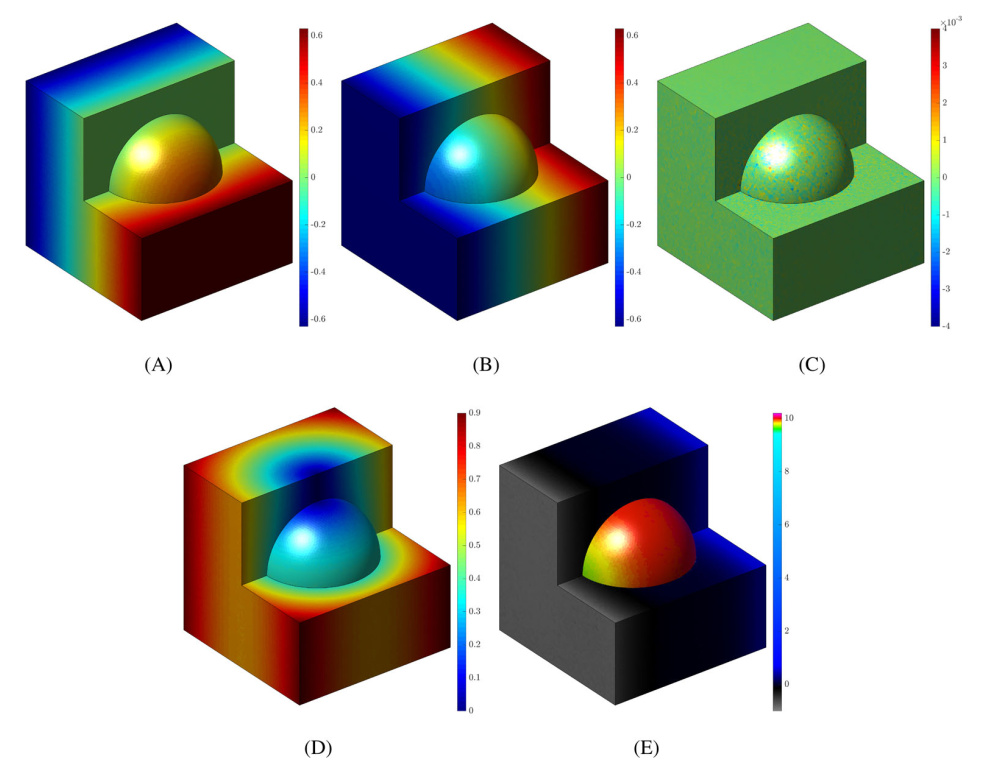
\includegraphics[width=15cm]{images/mms/sedu23b}\\
{\captionfont Taken from \cite{sedu23}. From left to right: 
$u$, $v$, $w$, $|\vec\upnu|$, $p$, for $\eta_1=1$ and $\eta=10^{2}.$}
\end{center}



